
\documentclass[a4paper]{article}
\usepackage{graphics}                 % Packages to allow inclusion of graphics
\usepackage[pdftex]{graphicx}
\usepackage{fancyhdr}
\usepackage[figuresright]{rotating}


% Margini
\setlength{\textwidth} {170mm}
\setlength{\textheight}{240mm}      %Altezza testo 227 mm
%\setlength{\topmargin} {0.1mm}

\setlength{\evensidemargin}{-5mm} %Margini per l'opzione twoside
\setlength{\oddsidemargin} {-5mm}
\setlength{\topmargin}{-10mm}


%\VignetteIndexEntry{Fig1ElamirSeheult} 


\title{Figure 1 in Elamir and Seheult (2004)}
\author{Alberto Viglione}

\usepackage{/usr/local/lib/R/share/texmf/Sweave}
\begin{document}
\maketitle




First of all load the library:
\begin{Schunk}
\begin{Sinput}
> library(nsRFA)
\end{Sinput}
\end{Schunk}
and generate the samples from the Normal distribution:
\begin{Schunk}
\begin{Sinput}
> Nsim = 1000
> n = 60
\end{Sinput}
\end{Schunk}
\begin{Schunk}
\begin{Sinput}
> campsimulati <- rnorm(n * Nsim)
\end{Sinput}
\end{Schunk}
\begin{Schunk}
\begin{Sinput}
> campsimulati <- matrix(campsimulati, ncol = n)
\end{Sinput}
\end{Schunk}
Then calculate $l_3$ and $SE(l_3)$:
\begin{Schunk}
\begin{Sinput}
> lmom <- t(apply(campsimulati, 1, Lmoments))
> vlmom <- t(apply(campsimulati, 1, varLmoments, matrix = FALSE))
> l3 <- lmom[, "lca"] * lmom[, "l2"]
> sl3 <- sqrt(vlmom[, "var.l3"])
\end{Sinput}
\end{Schunk}
\begin{Schunk}
\begin{Sinput}
> l3gaussian <- l3/sl3
\end{Sinput}
\end{Schunk}
and plot the results:
\begin{Schunk}
\begin{Sinput}
> qqnorm(l3gaussian, main = "Normal Q-Q Plot for Gaussian samples")
> qqline(l3gaussian)
\end{Sinput}
\end{Schunk}

Repeat the same procedure for the Student distribution:
\begin{Schunk}
\begin{Sinput}
> campsimulati <- rt(n * Nsim, df = 5)
\end{Sinput}
\end{Schunk}
\begin{Schunk}
\begin{Sinput}
> campsimulati <- matrix(campsimulati, ncol = n)
> lmom <- t(apply(campsimulati, 1, Lmoments))
> vlmom <- t(apply(campsimulati, 1, varLmoments, matrix = FALSE))
> l3 <- lmom[, "lca"] * lmom[, "l2"]
> sl3 <- sqrt(vlmom[, "var.l3"])
\end{Sinput}
\end{Schunk}
\begin{Schunk}
\begin{Sinput}
> l3student <- l3/sl3
\end{Sinput}
\end{Schunk}
the Cauchy distribution:
\begin{Schunk}
\begin{Sinput}
> campsimulati <- rcauchy(n * Nsim)
\end{Sinput}
\end{Schunk}
\begin{Schunk}
\begin{Sinput}
> campsimulati <- matrix(campsimulati, ncol = n)
> lmom <- t(apply(campsimulati, 1, Lmoments))
> vlmom <- t(apply(campsimulati, 1, varLmoments, matrix = FALSE))
> l3 <- lmom[, "lca"] * lmom[, "l2"]
> sl3 <- sqrt(vlmom[, "var.l3"])
\end{Sinput}
\end{Schunk}
\begin{Schunk}
\begin{Sinput}
> l3cauchy <- l3/sl3
\end{Sinput}
\end{Schunk}
and the Uniform distribution:
\begin{Schunk}
\begin{Sinput}
> campsimulati <- runif(n * Nsim)
\end{Sinput}
\end{Schunk}
\begin{Schunk}
\begin{Sinput}
> campsimulati <- matrix(campsimulati, ncol = n)
> lmom <- t(apply(campsimulati, 1, Lmoments))
> vlmom <- t(apply(campsimulati, 1, varLmoments, matrix = FALSE))
> l3 <- lmom[, "lca"] * lmom[, "l2"]
> sl3 <- sqrt(vlmom[, "var.l3"])
\end{Sinput}
\end{Schunk}
\begin{Schunk}
\begin{Sinput}
> l3unif <- l3/sl3
\end{Sinput}
\end{Schunk}

Plot the result:
\begin{figure}
\begin{center}
\begin{Schunk}
\begin{Sinput}
> layout(matrix(c(1, 2, 3, 4), 2, 2, byrow = TRUE))
> qqnorm(l3gaussian, main = "Normal Plot: Gaussian samples")
> qqline(l3gaussian)
> qqnorm(l3student, main = "Normal Plot: Student (df=5) samples")
> qqline(l3student)
> qqnorm(l3cauchy, main = "Normal Plot: Cauchy samples")
> qqline(l3cauchy)
> qqnorm(l3unif, main = "Normal Plot: Uniform samples")
> qqline(l3unif)
\end{Sinput}
\end{Schunk}
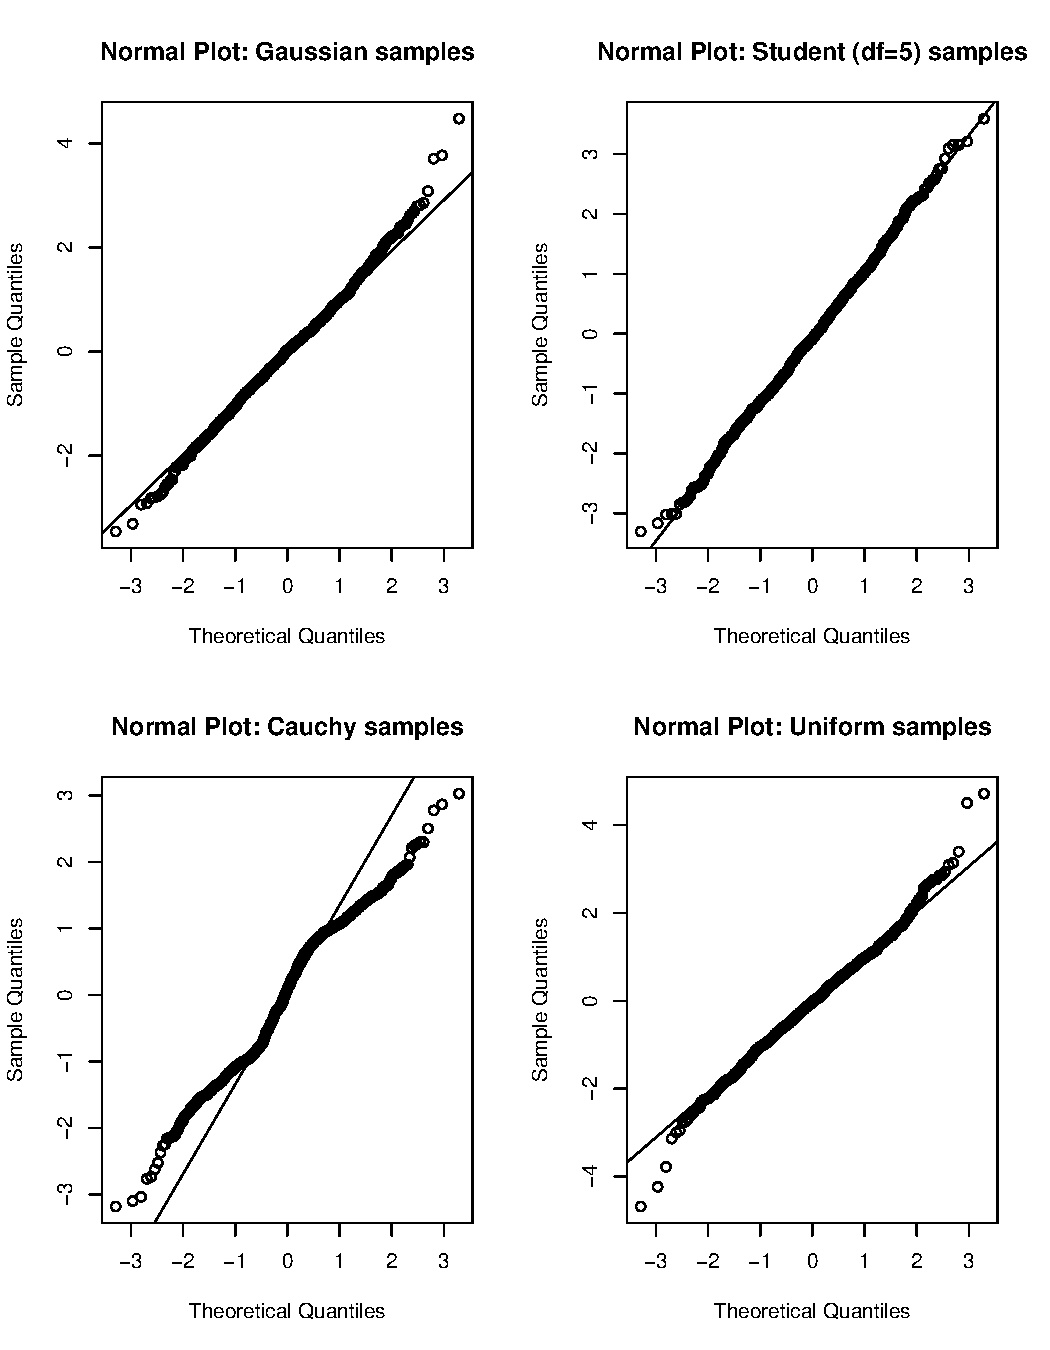
\includegraphics{Fig1ElamirSeheult-017}
\end{center}
\caption{Normal quantile plots and added line for $N=1000$ simulated values of $l_3/SE(l_3)$ from Gaussian, Student(5), Cauchy and Uniform samples of size $n=60$.}
\end{figure}
\end{document}

